\documentclass[aspectratio=169, 11pt]{beamer}

% ─── Theme & Colors ──────────────────────────────────────────────────────────
\usetheme{Madrid}
\usecolortheme{whale}
\definecolor{IITBlue}{RGB}{0, 51, 102}
\definecolor{AccentOrange}{RGB}{230, 126, 34}
\definecolor{LightBG}{RGB}{245, 248, 252}
\setbeamercolor{palette primary}{bg=IITBlue, fg=white}
\setbeamercolor{palette secondary}{bg=IITBlue!80, fg=white}
\setbeamercolor{palette tertiary}{bg=IITBlue!60, fg=white}
\setbeamercolor{structure}{fg=IITBlue}
\setbeamercolor{title}{fg=white, bg=IITBlue}
\setbeamercolor{frametitle}{fg=white, bg=IITBlue}
\setbeamercolor{block title}{bg=IITBlue, fg=white}
\setbeamercolor{block body}{bg=LightBG}
\setbeamercolor{block title alerted}{bg=AccentOrange, fg=white}
\setbeamercolor{block body alerted}{bg=AccentOrange!10}
\setbeamercolor{item}{fg=IITBlue}
\setbeamertemplate{navigation symbols}{}
\setbeamertemplate{footline}{
  \leavevmode\hbox{%
    \begin{beamercolorbox}[wd=.33\paperwidth,ht=2.5ex,dp=1ex,center]{palette primary}
      \usebeamerfont{author in head/foot}\insertshortauthor
    \end{beamercolorbox}%
    \begin{beamercolorbox}[wd=.34\paperwidth,ht=2.5ex,dp=1ex,center]{palette secondary}
      \usebeamerfont{title in head/foot}\insertshorttitle
    \end{beamercolorbox}%
    \begin{beamercolorbox}[wd=.33\paperwidth,ht=2.5ex,dp=1ex,right]{palette tertiary}
      \usebeamerfont{date in head/foot}\insertframenumber{} / \inserttotalframenumber\hspace*{2ex}
    \end{beamercolorbox}%
  }
}

% ─── Packages ────────────────────────────────────────────────────────────────
\usepackage{amsmath, amssymb}
\usepackage{booktabs}
\usepackage{graphicx}
\usepackage{tikz}
\usetikzlibrary{arrows.meta, positioning, decorations.pathreplacing, calc, shapes.geometric}
\usepackage{xcolor}
\usepackage{fontenc}
\usepackage[T1]{fontenc}

% ─── Title Info ──────────────────────────────────────────────────────────────
\title[EVRP with Dynamic Pricing]{Deep Reinforcement Learning for Electric Vehicle Routing \\ under Dynamic Time-of-Use Energy Pricing}
\subtitle{B.Tech Project --- Midterm Evaluation}
\author[Chaitanya Saagar]{Chaitanya Saagar \\ \small Roll No: 2301CS77}
\institute[]{Supervisor: Prof.\ Samrat Mondal \\ Department of Computer Science \& Engineering}
\date{October 2026}

\begin{document}

% ═══════════════════════════════════════════════════════════════════════════════
% TITLE SLIDE
% ═══════════════════════════════════════════════════════════════════════════════
{
\setbeamertemplate{footline}{}
\begin{frame}
\titlepage
\end{frame}
}

% ═══════════════════════════════════════════════════════════════════════════════
% SLIDE 1: INTRODUCTION
% ═══════════════════════════════════════════════════════════════════════════════
\begin{frame}{Introduction}

\begin{columns}[T]
\begin{column}{0.55\textwidth}

\begin{block}{The Electric Fleet Revolution}
\begin{itemize}
    \item Last-mile delivery fleets are rapidly transitioning from ICE to \textbf{electric vehicles (EVs)}.
    \item EVs introduce \textbf{range constraints} (finite battery) and \textbf{mandatory charging stops} --- absent in classical VRP.
    \item Electricity prices are \textbf{not static}: modern smart grids use \textbf{Time-of-Use (ToU) pricing} that fluctuates hourly based on grid load.
\end{itemize}
\end{block}

\vspace{0.3em}
\begin{alertblock}{Key Insight}
\textit{When} you charge matters as much as \textit{where} you charge.  A vehicle that times its stops to exploit cheap pricing windows can save \textbf{30--60\%} on energy costs.
\end{alertblock}

\end{column}
\begin{column}{0.42\textwidth}

\centering
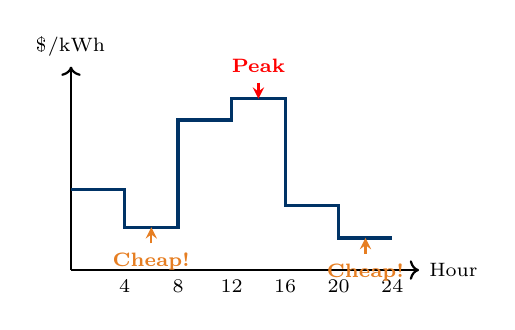
\begin{tikzpicture}[scale=0.68, every node/.style={font=\scriptsize}]
    % Price curve
    \draw[->, thick] (0,0) -- (6.5,0) node[right] {Hour};
    \draw[->, thick] (0,0) -- (0,3.8) node[above] {\$/kWh};

    % Step function prices
    \draw[IITBlue, very thick]
        (0,1.5) -- (1,1.5) -- (1,0.8) -- (2,0.8) -- (2,2.8) -- (3,2.8)
        -- (3,3.2) -- (4,3.2) -- (4,1.2) -- (5,1.2) -- (5,0.6) -- (6,0.6);

    % Labels
    \node[below] at (1,0) {4};
    \node[below] at (2,0) {8};
    \node[below] at (3,0) {12};
    \node[below] at (4,0) {16};
    \node[below] at (5,0) {20};
    \node[below] at (6,0) {24};

    % Annotations
    \draw[AccentOrange, thick, ->, >=stealth] (1.5,0.5) -- (1.5,0.8);
    \node[AccentOrange, below] at (1.5,0.5) {\textbf{Cheap!}};

    \draw[red, thick, ->, >=stealth] (3.5,3.5) -- (3.5,3.2);
    \node[red, above] at (3.5,3.5) {\textbf{Peak}};

    \draw[AccentOrange, thick, ->, >=stealth] (5.5,0.3) -- (5.5,0.6);
    \node[AccentOrange, below] at (5.5,0.3) {\textbf{Cheap!}};
\end{tikzpicture}

\vspace{0.6em}
{\footnotesize \textit{Time-of-Use electricity pricing:} \\
the same station costs 4$\times$ more \\ at peak vs.\ off-peak hours.}

\end{column}
\end{columns}

\end{frame}

% ═══════════════════════════════════════════════════════════════════════════════
% SLIDE 2: PROBLEM STATEMENT
% ═══════════════════════════════════════════════════════════════════════════════
\begin{frame}{Problem Statement}

\begin{block}{The Electric Vehicle Routing Problem (EVRP) with Dynamic Pricing}
Given a depot, a set of customers, and charging stations with \textbf{time-varying electricity prices}, find the route and charging schedule that \textbf{minimizes total operational cost} (distance wear + energy cost) while satisfying:
\end{block}

\vspace{0.4em}

\begin{columns}[T]
\begin{column}{0.48\textwidth}

\textbf{Hard Constraints:}
\begin{enumerate}
    \item Every customer visited exactly once
    \item Battery $> 0$ at all times (no stranding)
    \item Vehicle returns to the depot
\end{enumerate}

\vspace{0.5em}

\textbf{Objective Function:}
\[
\min \sum_{(i,j) \in \mathcal{R}} \underbrace{c_d \cdot d_{ij}}_{\text{distance cost}} + \sum_{k \in \mathcal{S}} \underbrace{p_k(t_k) \cdot e_k}_{\text{charging cost}}
\]

{\small where $p_k(t_k)$ = price at station $k$ at arrival time $t_k$, \\ $e_k$ = energy charged (kWh)}

\end{column}
\begin{column}{0.48\textwidth}

\textbf{Why This Is Hard:}

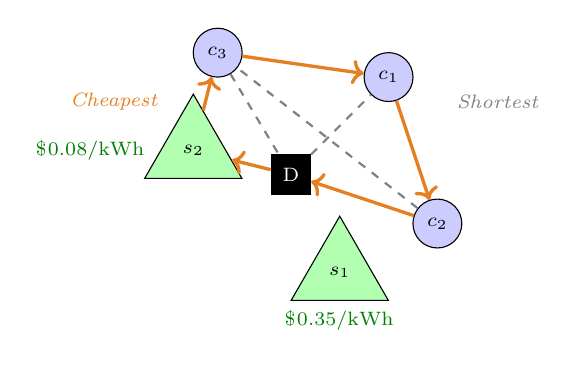
\begin{tikzpicture}[scale=0.62, every node/.style={font=\scriptsize}]
    % Nodes
    \node[draw, fill=black, text=white, minimum size=0.5cm] (D) at (0,0) {D};
    \node[draw, circle, fill=blue!20, minimum size=0.4cm] (C1) at (2,2) {$c_1$};
    \node[draw, circle, fill=blue!20, minimum size=0.4cm] (C2) at (3,-1) {$c_2$};
    \node[draw, circle, fill=blue!20, minimum size=0.4cm] (C3) at (-1.5,2.5) {$c_3$};
    \node[draw, regular polygon, regular polygon sides=3, fill=green!30, minimum size=0.5cm] (S1) at (1,-2) {$s_1$};
    \node[draw, regular polygon, regular polygon sides=3, fill=green!30, minimum size=0.5cm] (S2) at (-2,0.5) {$s_2$};

    % Shortest path (gray, dashed)
    \draw[gray, dashed, thick] (D) -- (C1) -- (C2) -- (C3) -- (D);
    \node[gray, right] at (3.2, 1.5) {\textit{Shortest}};

    % Smart path (orange)
    \draw[AccentOrange, very thick, ->] (D) -- (S2);
    \draw[AccentOrange, very thick, ->] (S2) -- (C3);
    \draw[AccentOrange, very thick, ->] (C3) -- (C1);
    \draw[AccentOrange, very thick, ->] (C1) -- (C2);
    \draw[AccentOrange, very thick, ->] (C2) -- (D);
    \node[AccentOrange, left] at (-2.5, 1.5) {\textit{Cheapest}};

    % Price labels
    \node[green!50!black, below] at (1,-2.6) {\$0.35/kWh};
    \node[green!50!black, left] at (-2.8,0.5) {\$0.08/kWh};
\end{tikzpicture}

\vspace{0.3em}
\begin{itemize}
    \item The \textbf{shortest route} may hit expensive charging windows
    \item The \textbf{cheapest route} deliberately detours to catch low prices
    \item Search space: $O\!\left(\frac{(N\!+\!M)!}{(M\!-\!k)!}\right)$ --- \textbf{factorial explosion}
\end{itemize}

\end{column}
\end{columns}

\end{frame}

% ═══════════════════════════════════════════════════════════════════════════════
% SLIDE 3: SOLUTION METHODOLOGY
% ═══════════════════════════════════════════════════════════════════════════════
\begin{frame}{Solution Methodology}

\begin{columns}[T]
\begin{column}{0.50\textwidth}

\begin{block}{Phase 1: Rule-Based Heuristic (Current Work)}
A two-phase construction + improvement solver:
\begin{enumerate}
    \item \textbf{Multi-seed construction:} Generate $N\!+\!1$ candidate customer orderings via nearest-neighbour from each starting point
    \item \textbf{Optimal station insertion:} For each ordering, simulate the drive and insert charging stops that minimize:
    \[
    \text{score}(s) = \underbrace{\Delta d \cdot c_d}_{\text{detour cost}} + \underbrace{p_s(t_{\text{arr}}) \cdot e}_{\text{charge cost}}
    \]
    \item \textbf{Opportunistic charging:} If a nearby station's price $< 0.65 \times \bar{p}$ and savings outweigh detour, charge preemptively
    \item \textbf{2-opt improvement:} Swap customer pairs, re-simulate, keep improvements
\end{enumerate}
\end{block}

\end{column}
\begin{column}{0.47\textwidth}

\begin{block}{Phase 2: Deep RL Agent (Planned)}
Formulate as a Markov Decision Process:
\vspace{0.3em}

\renewcommand{\arraystretch}{1.3}
\begin{tabular}{@{}l p{4.5cm}@{}}
\toprule
\textbf{State} $S_t$ & Location, battery SoC, unvisited mask, \textbf{price forecast} \\
\textbf{Action} $A_t$ & Next node to visit \\
\textbf{Reward} $R_t$ & $-w_1 d_{ij} + w_2(\bar{p} - p_t) \cdot e$ for arbitrage; $-1000$ for SLA/battery violations \\
\bottomrule
\end{tabular}

\vspace{0.5em}
\textbf{Algorithm:} PPO with MLP policy \\
\textbf{Key innovation:} Rolling price forecast vector in the observation space enables the agent to learn temporal arbitrage
\end{block}

\vspace{0.3em}
\textbf{Complexity:} Rule-based $O(N^3)$ vs.\ brute-force $O(N!)$ \\ RL inference: $O(1)$ per decision step

\end{column}
\end{columns}

\end{frame}

% ═══════════════════════════════════════════════════════════════════════════════
% SLIDE 4: RESULTS
% ═══════════════════════════════════════════════════════════════════════════════
\begin{frame}{Results}

\begin{columns}[T]
\begin{column}{0.48\textwidth}

\begin{block}{Toy World (5 customers, 4 stations)}
Brute-force verifiable --- 557,400 paths enumerated
\end{block}

\vspace{0.3em}
\renewcommand{\arraystretch}{1.25}
\begin{tabular}{@{}l r r@{}}
\toprule
\textbf{Method} & \textbf{Cost (\$)} & \textbf{vs Optimal} \\
\midrule
Brute-force optimal & 17.10 & --- \\
\textcolor{AccentOrange}{\textbf{Rule-based smart}} & \textcolor{AccentOrange}{\textbf{18.48}} & \textcolor{AccentOrange}{\textbf{+8.1\%}} \\
Greedy baseline & 42.69 & +149.7\% \\
\bottomrule
\end{tabular}

\vspace{0.6em}

\begin{block}{Scaled World (15 customers, 8 stations)}
Brute-force impossible ($\sim\!10^{17}$ paths)
\end{block}

\vspace{0.3em}
\renewcommand{\arraystretch}{1.25}
\begin{tabular}{@{}l r r r@{}}
\toprule
\textbf{Method} & \textbf{Cost} & \textbf{Charges} & \textbf{Savings} \\
\midrule
\textcolor{AccentOrange}{\textbf{Rule-based}} & \textcolor{AccentOrange}{\textbf{\$54.12}} & \textcolor{AccentOrange}{\textbf{10}} & \textcolor{AccentOrange}{\textbf{32.9\%}} \\
Greedy & \$80.68 & 4 & --- \\
\bottomrule
\end{tabular}

\end{column}
\begin{column}{0.48\textwidth}

\begin{center}
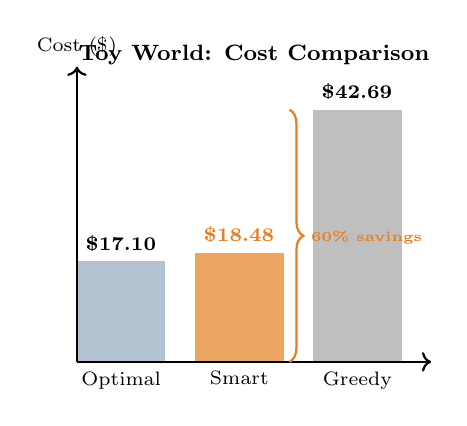
\begin{tikzpicture}[scale=0.75]
    % Bar chart
    \fill[IITBlue!30] (0,0) rectangle (1.5, 1.71);
    \fill[AccentOrange!70] (2,0) rectangle (3.5, 1.85);
    \fill[gray!50] (4,0) rectangle (5.5, 4.27);

    \node[below, font=\scriptsize] at (0.75, 0) {Optimal};
    \node[below, font=\scriptsize] at (2.75, 0) {Smart};
    \node[below, font=\scriptsize] at (4.75, 0) {Greedy};

    \node[above, font=\scriptsize\bfseries] at (0.75, 1.71) {\$17.10};
    \node[above, font=\scriptsize\bfseries, AccentOrange] at (2.75, 1.85) {\$18.48};
    \node[above, font=\scriptsize\bfseries] at (4.75, 4.27) {\$42.69};

    \draw[->, thick] (0,0) -- (6,0);
    \draw[->, thick] (0,0) -- (0,5) node[above, font=\scriptsize] {Cost (\$)};

    \node[font=\footnotesize\bfseries] at (3, 5.2) {Toy World: Cost Comparison};

    % Savings annotation
    \draw[AccentOrange, thick, decorate, decoration={brace, amplitude=5pt, mirror}]
        (3.6, 0) -- (3.6, 4.27);
    \node[AccentOrange, right, font=\tiny\bfseries] at (3.8, 2.1) {60\% savings};
\end{tikzpicture}
\end{center}

\vspace{0.4em}

\begin{alertblock}{Key Takeaway}
The rule-based solver captures \textbf{92\% of the theoretical optimum} in the toy world, and saves \textbf{33\%} over greedy in the scaled world --- by charging more frequently at cheaper stations, even at the cost of extra distance.
\end{alertblock}

\end{column}
\end{columns}

\end{frame}

% ═══════════════════════════════════════════════════════════════════════════════
% SLIDE 5: FUTURE PLAN
% ═══════════════════════════════════════════════════════════════════════════════
\begin{frame}{Future Plan}

\begin{columns}[T]
\begin{column}{0.55\textwidth}

\begin{block}{Remaining Work (Nov 2026 -- Mar 2027)}
\begin{enumerate}
    \item \textbf{Custom Gymnasium Environment} \\
    {\small Implement the EVRP as a \texttt{gymnasium.Env} with action masking, composite state space (location + SoC + price forecast), and shaped reward function}

    \vspace{0.3em}
    \item \textbf{Price Forecasting Module} \\
    {\small Lightweight LSTM/AR model for short-horizon (1--2h) price prediction, embedded in the RL observation space}

    \vspace{0.3em}
    \item \textbf{PPO Training Pipeline} \\
    {\small Train with Stable-Baselines3, \texttt{MultiInputPolicy}, curriculum learning (small $\to$ large worlds)}

    \vspace{0.3em}
    \item \textbf{Comprehensive Benchmarking} \\
    {\small DRL agent vs.\ rule-based vs.\ greedy vs.\ OR-Tools, across multiple world sizes and price volatility levels}
\end{enumerate}
\end{block}

\end{column}
\begin{column}{0.42\textwidth}

\begin{center}
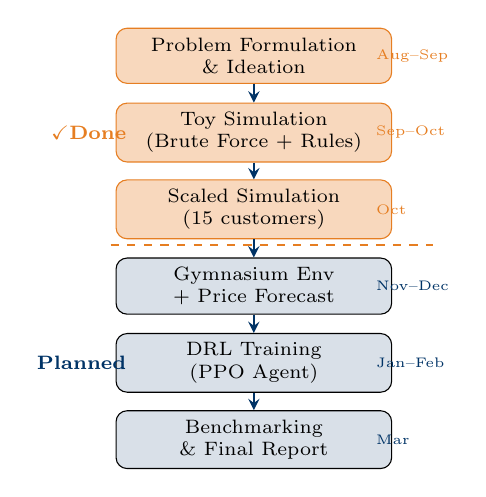
\begin{tikzpicture}[
    scale=0.65,
    phase/.style={draw, rounded corners, fill=IITBlue!15, minimum width=3.5cm, minimum height=0.7cm, font=\scriptsize, align=center},
    done/.style={phase, fill=AccentOrange!30, draw=AccentOrange},
    arr/.style={->, >=stealth, thick, IITBlue}
]
    \node[done] (p1) at (0, 0) {Problem Formulation \\ \& Ideation};
    \node[done] (p2) at (0, -1.5) {Toy Simulation \\ (Brute Force + Rules)};
    \node[done] (p3) at (0, -3.0) {Scaled Simulation \\ (15 customers)};
    \node[phase] (p4) at (0, -4.5) {Gymnasium Env \\ + Price Forecast};
    \node[phase] (p5) at (0, -6.0) {DRL Training \\ (PPO Agent)};
    \node[phase] (p6) at (0, -7.5) {Benchmarking \\ \& Final Report};

    \draw[arr] (p1) -- (p2);
    \draw[arr] (p2) -- (p3);
    \draw[arr] (p3) -- (p4);
    \draw[arr] (p4) -- (p5);
    \draw[arr] (p5) -- (p6);

    % Timeline
    \node[right, font=\tiny, AccentOrange] at (2.2, 0) {Aug--Sep};
    \node[right, font=\tiny, AccentOrange] at (2.2, -1.5) {Sep--Oct};
    \node[right, font=\tiny, AccentOrange] at (2.2, -3.0) {Oct};
    \node[right, font=\tiny, IITBlue] at (2.2, -4.5) {Nov--Dec};
    \node[right, font=\tiny, IITBlue] at (2.2, -6.0) {Jan--Feb};
    \node[right, font=\tiny, IITBlue] at (2.2, -7.5) {Mar};

    % Done marker
    \node[AccentOrange, font=\scriptsize\bfseries, left] at (-2.3, -1.5) {\checkmark Done};
    \draw[AccentOrange, dashed, thick] (-2.8, -3.7) -- (3.5, -3.7);
    \node[IITBlue, font=\scriptsize\bfseries, left] at (-2.3, -6.0) {Planned};
\end{tikzpicture}
\end{center}

\end{column}
\end{columns}

\end{frame}

\end{document}
